\documentclass[a4paper]{article}


\usepackage[utf8]{inputenc}
\usepackage[T1]{fontenc}
\usepackage{textcomp}
\usepackage{mathtools,amssymb,amsthm}
\usepackage[top=2.5cm,bottom=2.5cm,right=2.5cm,left=2.5cm]{geometry}
\usepackage[francais]{babel}
\usepackage{appendix}

%================image=================
\usepackage{graphicx}
\graphicspath{{figures/}}
\renewcommand{\listfigurename}{Table des figures}

%============header and foot============
\usepackage{fancyhdr}
\pagestyle{fancy}
\renewcommand\headrulewidth{1pt}
\fancyhead[L]{\bfseries Algorithmique Numérique}
\fancyhead[R]{
\includegraphics[scale=0.05]{./img/prepisima.png}}
\fancyfoot[L]{SABIER Corentin et CHASSAGNOL Rémi}
\fancyfoot[R]{2020-2021}

%=================other================
\renewcommand{\contentsname}{Table des matières}

%=================code=================
\usepackage{verbatim}
\usepackage{listings}
\usepackage{color}
\usepackage[table]{xcolor}

%==============code settings==========
\definecolor{darkWhite}{rgb}{1,1,1}
\definecolor{myred}{rgb}{1,0.22,0.22}
\definecolor{mypurple}{rgb}{0.74,0.36,0.97}
\lstset{
  mathescape,
  aboveskip=3mm,
  belowskip=-2mm,
  backgroundcolor=\color{darkWhite},
  basicstyle=\ttfamily\footnotesize,
  breakatwhitespace=false,
  breaklines=true,
  captionpos=b,
  commentstyle=\color{myred},
  deletekeywords={...},
  escapeinside={\%*}{*)},
  extendedchars=true,
  framexleftmargin=16pt,
  framextopmargin=3pt,
  framexbottommargin=6pt,
  frame=tb,
  keepspaces=true,
  keywordstyle=\color{mypurple},
  language=C,
  morekeywords={*,...},
  numbers=left,
  numbersep=10pt,
  numberstyle=\tiny\color{black},
  rulecolor=\color{black},
  showspaces=false,
  showstringspaces=false,
  showtabs=false,
  stepnumber=1,
  stringstyle=\color{gray},
  tabsize=4,
  title=\lstname,
}

\begin{document}

%===========Page de guarde============
\begin{titlepage}
  \begin{center}
    
    \begin{figure}[h]
      \centering
      
\includegraphics[scale=0.3]{./img/logo.png}
      \caption{logo uca}
      \label{uca}
    \end{figure}
    \\[1.5cm]
    \textsc{\LARGE TP}\\[0.5cm]
    
    {\huge \bfseries Algorithmique Numérique\\[0.4cm]}

    \begin{figure}[h]
      \centering
      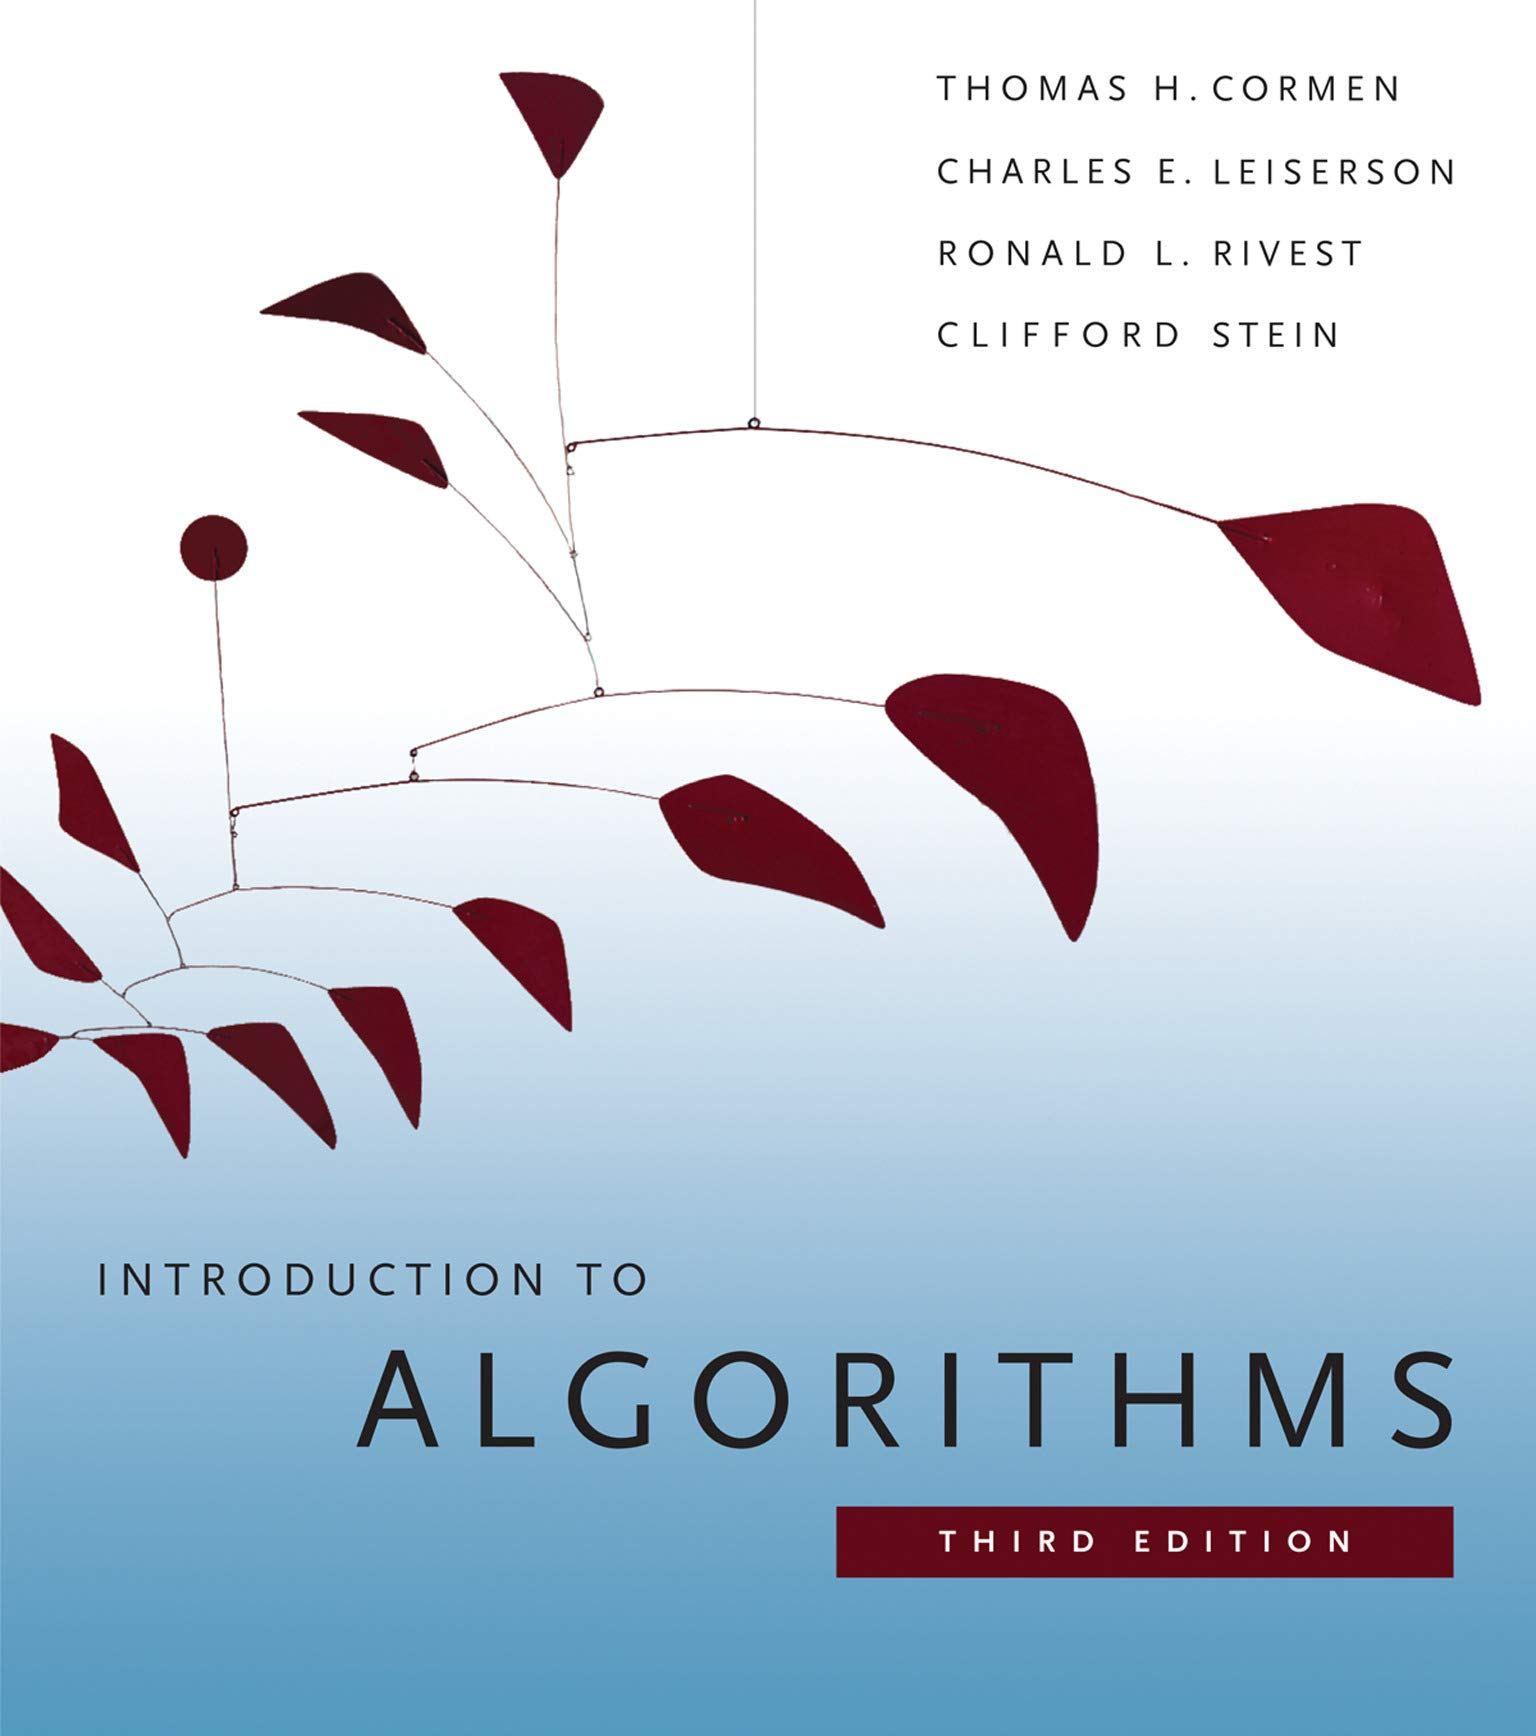
\includegraphics[scale=0.2]{./img/cormen.jpg}
      \caption{Cormen}
    \end{figure}

    \begin{minipage}{0.9\textwidth}
      \begin{flushleft} \large
        SABIER Corentin et CHASSAGNOL Rémi\\
        année 2020-2021\\[2cm]
      \end{flushleft}
    \end{minipage}

    \begin{minipage}{0.9\textwidth}
      \begin{flushright} \large
        \emph{Professeur:} CHORFI Amina\\
      \end{flushright}
    \end{minipage}

    \textsc{24 octobre 2020}

  \end{center}
\end{titlepage}

\clearpage

\tableofcontents

\clearpage

\section{Algorithmes directes}

\subsection{Gauss}

\subsubsection{Principe}

Le principe de cette méthode est de manipuler une matrice \textbf{A} de coefficients du système linéaire, de sorte qu'elle devienne triangulaire supérieure. Les coefficients $a_{ii} = 1$ tels que $i \in [0,n[$ . Ensuite par substitution des inconnues, on obtient la matrice solution facilement grâce au système échelonné.

\[
A \cdot X = B \text{  où  } A = \begin{pmatrix} 
a_{11} & .  & . & . & a_{1n}\\ 
.      & .  & . & . & . \\ 
.      & .  & . & . & . \\ 
.      & .  & . & . & . \\
a_{n1} & .  & . & . & a_{nn} \\  
\end{pmatrix}
\longrightarrow
\begin{pmatrix} 
1      & a_{12}  & . & . & a_{1n}\\ 
0      & 1  	 & . & . & . \\ 
.      & .  	 & 1 & . & . \\ 
.      & .   	 & . & 1 & a_{n-1n} \\
0      & .  	 & . & 0 & 1 \\  
\end{pmatrix}
\]

\subsubsection{L'Algorithme du pivot de Gauss}

\begin{lstlisting}
$k := 0$;
Pour $j$ allant de $1$ a $p$ :
	Si il existe $i \in [k+1,n]$ tel que $a_{ij} \neq 0$ alors : 
			
			$k:= k + 1$;
			$q:=$ choix$(i \in [k,n])$ tel que $a_{ij} \neq 0)$;
			$L_q \leftarrow \frac{1}{a_{qj}}L_q$;
			
			Si $k \neq q$ alors :
				$L_k \leftrightarrow L_q$;
			
			Pour $i$ allant de $k + 1$ a $n$;
				$L_i \leftarrow L_i - a_{ij}L_k$;
						
\end{lstlisting}

Dans l'ordre l'algorithme fait :

\begin{itemize}
	\item Ligne 1 : indice de ligne du pivot;
	\item Ligne 2 : indice de colonne;
	\item Ligne 3 : test existence du prochain pivot;
	\item Ligne 5 : mise à jour de l'indice de ligne du pivot;
	\item Ligne 6 : choix du nouveau pivot;
	\item Ligne 7 : normalisation;
	\item Ligne 10: mise du pivot à la bonne place;
	\item Ligne 12: élimination des valeurs sous le pivot;						
\end{itemize} 

\subsubsection{Les fonctions}

Pour simplifier la lisibilité du programme certaines opérations sont gérées par des fonctions annexes telles que :
\newline
\begin{itemize}
	\item La normalisation (fonction "\textit{normaLigne}")
	\item L'échange de deux lignes (fonction "\textit{echangeLigne}")
	\item La soustraction entre deux lignes (fonction "\textit{soustractionLignes}")
	\item La résolution du système, une fois la matrice échelonnée (fonction "\textit{resolution}")
\end{itemize}
\clearpage
\begin{lstlisting}
	void normaLigne(float ** A, float * B, int n, int q, int j)
	{
		int ji;
		float tmp = A[q][j];
		
		"Division de chaque elements de la ligne q de matrice A et B:"
		for(ji = q;ji < n;ji++)
		{
			iteration++;
			A[q][ji] = A[q][ji] / tmp;
		}
		B[q] = B[q]/tmp;: 
	}
\end{lstlisting}

NormaLigne : Normalise une ligne de la matrice, ici la ligne du pivot \textbf{q}.

\begin{lstlisting}
	void echangeLigne(float ** A, float * B, int n, int q, int k)
	{
		float tmp;
		int j;
		for (j = 0; j<n ;j++)
		{
			iteration++;
			tmp     = A[k][j];
			A[k][j] = A[q][j];
			A[q][j] = tmp;
		} 
		
		tmp  = B[k] ;
		B[k] = B[q];
		B[q] = tmp;
	}
\end{lstlisting}

EchangeLigne : Echange les valeurs de la ligne \textbf{q} et \textbf{k}.

\begin{lstlisting}
	void soustractionLignes(float ** A, float * B, int n, int i, int j, int k)
	{
		int ji;
		float tmp = A[i][j];
		
		for(ji = 0; ji < n; ji++)
		{
			iteration++;
			A[i][ji] = A[i][ji] - tmp*A[k][ji];
		}
		B[i] -= tmp * B[k];
	}
\end{lstlisting}

SoustractionLignes : Soustrait les valeurs de la ligne \textbf{k} aux valeurs de la ligne \textit{i} de sorte que la valeur sous le pivot (à la colonne \textbf{j}) devienne nulle.
\newline
\textit{Note : ne pas prendre en compte la variable} \textbf{iteration} \textit{, elle sert à retourner la complexité pratique du programme.}
\clearpage
\begin{lstlisting}
	float * resolution(float ** A, float * B, int n)
	{
		float * X = (float *)malloc(n*sizeof(float)); 			
		float somme;
		
		for (int i = n-1; i>=0; i--)			"indice de la ligne"
		{
			iteration++;
			somme = 0;
			for (int j = n-1; j>i; j--)			"indice de la colonne"
			{
				somme += A[i][j]*X[j];
			}
			X[i] = (B[i]-somme);
		}
		return X;
	}
\end{lstlisting}

Resolution : Renvoie la matrice solution du système linéaire. Elle parcours la matrice \textbf{A} depuis le bas de la diagonale (en $a_{nn}$). puis remonte jusqu'à l'autre extrémité.
A ce stade, pour chaque ligne $i$ on a l'inconnue $x_i$ telle que :
\[x_i = b_i - \sum_{k = i+1}^{n}a_{ik}x_k\]


\subsubsection{Les tests}

Tout les systèmes seront tels que :\\
\[
A \cdot X = 
\begin{pmatrix} 
1  \\ 
1  \\ 
1  \\ 
1  \\
\end{pmatrix}
\]
\\
\textbf{\underline{\large{Ding Dong :}}}
\\
\\
\begin{center}
	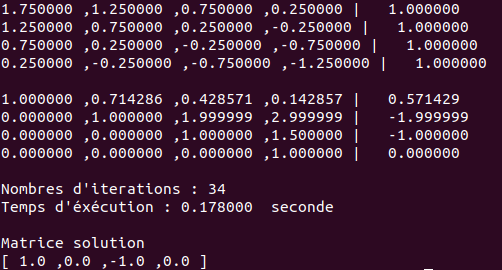
\includegraphics[scale=0.5]{./img/gauss/TestDingDong.png} \\
\end{center}

Ici on a Ding Dong carré de dimension 4, et le système échelonné ci-dessus.
Le programme trouve la matrice solution attendue.
On remarque que la méthode a une complexité pratique de 34 opérations sur ce système, et qu'il le résout en 0.178 seconde environ.
\\
La fonction d'erreur est nulle (on trouve les valeurs exactes).
Résolvons le même système en faisant varier les valeurs dans b de +0.005, on obtiens:
\\
\begin{center}
	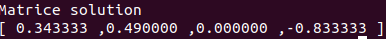
\includegraphics[scale=0.5]{./img/gauss/dingdong005.png} \\
\end{center}

Les valeurs sont assez proches, mais les valeurs à 1 et -1 se retrouvent plus proches de 0 et inversement, les valeurs proches de 0 en sont encore plus éloignées que ces dernières.
La méthode n'est donc pas stable pour ce système linéaire.
\\
\\
\textbf{\underline{\large{Moler :}}}
\\
\\
\begin{center}
	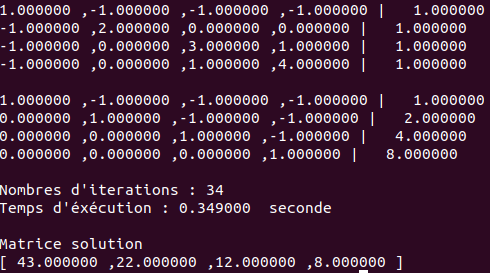
\includegraphics[scale=0.5]{./img/gauss/TestMoler.png} \\
\end{center}

Ici on a Ding Dong carré de dimension 4, et le système échelonné ci-dessus.
Le programme trouve la bonne solution.
La méthode a encore une complexité pratique de 34 opérations sur ce système, et qu'il le résout en 0.349 seconde environ.
\\
La fonction d'erreur est nulle (on trouve les valeurs exactes).
Résolvons le même système en faisant varier les valeurs dans b de +0.005, on obtient:
\\
\begin{center}
	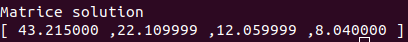
\includegraphics[scale=0.5]{./img/gauss/moler005.png} \\
\end{center}

Or les valeurs restent sensiblement identiques, ce qui indique que la méthode est stable sur ce système.
\\
\\
\textbf{\underline{\large{Franc :}}}
\\
\\
\begin{center}
	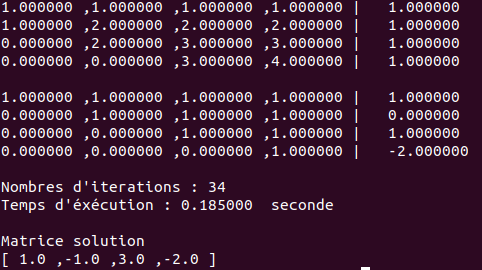
\includegraphics[scale=0.5]{./img/gauss/TestFranc.png} \\
\end{center}

Ici on a Ding Dong carré de dimension 4, et le système échelonné ci-dessus.
Le programme trouve la matrice solution attendue.
On remarque que la méthode a une complexité pratique de 34 opérations sur ce système, et qu'il le résout en 0.221 seconde environ.
\\
La fonction d'erreur est nulle (on trouve les valeurs exactes).\\
Résolvons le même système en faisant varier les valeurs dans b de +0.005, on obtient:
\\
\begin{center}
	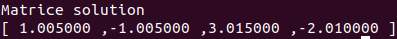
\includegraphics[scale=0.5]{./img/gauss/franc005.png} \\
\end{center}

Or les valeurs restent sensiblement identiques, ce qui indique que la méthode
est stable sur ce système linéaire également.

\clearpage

\subsection{Cholesky}

\subsubsection{Principe}

Le principe de cette méthode est de trouver une matrice $R$ telle que $A =
R^{T}R$ où $R$ est une matrice triangulaire supérieure et $R^{T}$ est la matrice
transposée de R. Le système $Ax = b$ peut donc se diviser en deux sous-systèmes
$R^{T}y = b$ et $Rx = y$. Cette méthode est légèrement plus rapide que celle de
Gauss avec une complexité de $\frac{n^{3}}{3}$ au lieu de $\frac{2n^{3}}{3}$,
cependant elle nécessite que la matrice soit définie positive.

\subsubsection{L'Algorithme}

L'algorithme qui permet de trouver la matrice $R$ est le suivant:

\begin{lstlisting}
  Pour $i$ allant de $1$ a $n$:
      $s = a_{ii} - \sum_{j=1}^{i-1}r_{ji}^{2}$
      Si $s \leqslant 0$ alors:
          arret("la matrice n'est pas definie positive")
      Sinon
         $r_{ii} = \sqrt{s}$
         Pour $j$ allant de $i+1$ a $n$:
            $r_{ij} = \frac{a_{ij} - \sum_{k=1}^{i-1}}{r_{ii}}$
\end{lstlisting}

Ensuite il suffit de résoudre les deux sous-systèmes ce qui se fait facilement
car la matrice est triangulaire.

\subsubsection{Les Variables}

Dans la fonction \textit{main} on initialise un matrice de taille
\textbf{LEN} qui est une constante pré-processeur. Les valeurs dans la matrice
dépendent de la constante \textbf{EXAMPLE} qui permet de déterminer
l’initialisation de la matrice via une fonction qui se situe dans le fichier
\textit{matrix.c}.

\begin{lstlisting}
  float *solus = malloc(LEN * sizeof(float));
  if (solus == NULL)
    exit(EXIT_FAILURE);
  float *b = malloc(LEN * sizeof(float));
  if (b == NULL)
    exit(EXIT_FAILURE);
  for (i = 0; i < LEN; i++) {
    b[i] = 1;
  }
  float **matrix = create_mat(LEN);
  mat(matrix, LEN, EXAMPLE);
  show(matrix, LEN);
  solver_cholesky(matrix, solus, b, LEN);
\end{lstlisting}

\clearpage

\subsubsection{Calcul de la matrice R}

On calcule la matrice $R$ (le tableau à deux dimensions \textit{r}) à
l'aide de la fonction nommée \textbf{make\_R} qui suit l'algorithme ci-dessus. A
noter que cette fonction renvoie une erreur si la matrice en entrée n'est pas
définie positive ce qui arrête le programme car le système n'est pas résolvable
avec cette méthode (en fait si la matrice n'est pas définie positive, la matrice
$R$ n'existe pas).

\begin{lstlisting}
void make_R(float **matrix, float **r, int n) {
  int i, j, k;   // loop var
  float sum = 0; // Used to calculate the sum of r_ki*r_kj
  float s;
  for (i = 0; i < n; i++) {
    s = matrix[i][i];
    for (j = 0; j < i; j++) {
      s -= r[j][i] * r[j][i];
    }
    if (s <= 0) {
      printf("La matrice n'est pas définie positive\n");
      exit(EXIT_FAILURE);
    } else {
      r[i][i] = sqrtf(s);
      for (j = (i + 1); j < n; j++) {
        sum = 0;
        for (k = 0; k < i; k++) {
          sum += r[k][i] * r[k][j];
        }
        r[i][j] = (matrix[i][j] - sum) / r[i][i];
      }
    }
  }
}
\end{lstlisting}

\subsubsection{Résolution des sous-systèmes}

Enfin la fonction \textbf{solver\_cholesky} résout les deux sous-systèmes de la
même manière qu'avec \textit{Gauss} sauf que les $a_{ii}$ ne sont pas forcement
égaux à 1 d'où la division par $a_{ii}$. De plus, dans le premier sous-système,
la matrice $R^{T}$ est triangulaire inférieure, la résolution se fait donc en
commençant par calculer la valeur de la première inconnue.

\begin{lstlisting}
void solver_cholesky(float **matrix, float *solus_x, float *b, int n) {
  int i, j;
  float tmp;
  float *solus_y = malloc(n * sizeof(float));
  /*Creation of the matrix  R:*/
  float **r = create_mat(n);
  mat_0(r, n);
  make_R(matrix, r, n);
  /*Resolution de R^T * y = b*/
  transpose(r, n);
  for (i = 0; i < n; i++) {
    tmp = b[i];
    for (j = 0; j < i; j++) {
      tmp -= solus_y[j] * r[i][j];
    }
    solus_y[i] = tmp / r[i][i];
  }
  /*Resolution R * x = y*/
  transpose(r, n);
  for (i = (n - 1); i >= 0; i--) {
    for (j = (n - 1); j > i; j--) {
      solus_y[i] -= solus_x[j] * r[i][j];
    }
    solus_x[i] = solus_y[i] / r[i][i];
  }
  /*FREE*/
  free(solus_y);
  for (i = 0; i < n; i++) {
    free(r[i]);
  }
  free(r);
}
\end{lstlisting}

Cette fonction fait appel à plusieurs autres fonctions:

\begin{itemize}
\item \textbf{create\_mat} qui retourne un tableau à deux dimensions de taille n
\item \textbf{mat\_0} qui remplit un tableau à deux dimensions de 0
\item \textbf{make\_R} vue ci-dessus
\item \textbf{transpose} qui transpose la matrice qui lui est donnée en argument
\end{itemize}

Résolution du premier sous\_système en détail:

\begin{lstlisting}
  for (i = 0; i < n; i++) {
    for (j = 0; j < i; j++) {
      b[i] -= solus_y[j] * r[i][j];
    }
    solus_y[i] = b[i] / r[i][i];
  }
\end{lstlisting}

Voici la matrice r (après avoir été transposée):\\

\begin{vmatrix}
  a_{11} & 0 & \cdots & \cdots & 0\\
  a_{21} & a_{22} & 0 & \cdots & 0\\
  \vdots & \cdots & \ddots & 0 & 0\\
  a_{n1} & \cdots & \cdots & \cdots & a_{nn}\\
\end{vmatrix}\\

Nous résolvons $Ry = b$ donc:

\[y_{i} = \frac{b_{i} - \sum_{j=1}^{i}}{a_{ii}}\]

Ce qui se fait à l'aide des deux boucles ci-dessus.\\

A noter que ce programme alloue plus de mémoire que le précédent à cause de
l'utilisation du tableau \textbf{r} ce qui pourrait être problématique si on
travaille avec des matrices de grande taille.

\subsubsection{Les Tests}

\begin{itemize}
\item Bord \\
  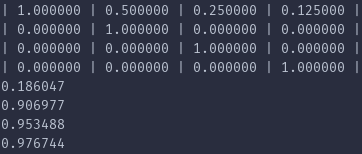
\includegraphics[scale=0.5]{./img/cholesky/bord.png} \\
  La méthode ne converge pas car la matrice n'est pas à diagonale dominante. Les
  vraies solutions du système sont:
  $x_{1} = \frac{1}{8} = 0.125 , x_{2} = 1 , x_{3} = 1 , x_{4} = 1$
\item Ding Dong \\
  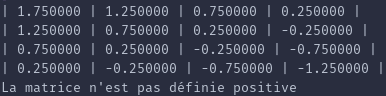
\includegraphics[scale=0.5]{./img/cholesky/ding_dong.png} \\
  Le programme retourne une erreur, en effet, la matrice n'est pas définie
  positive donc la méthode ne converge pas.
\item Matrice à diagonale dominante \\
  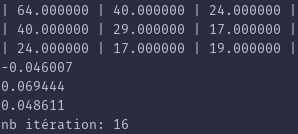
\includegraphics[scale=0.5]{./img/cholesky/chocho_test_final.png} \\
  Cette matrice est à diagonale dominante donc la méthode converge. La solution
  en valeur exacte est :
  \quad$x_{1} = \frac{-53}{1152} \approx -0.4600694444$,
  \quad$x-{2} = \frac{5}{72} \approx 0.06944444444$
  \quad$x_{3} = \frac{7}{144} = 0.048611111111$
  
  Ce qui est très proche de ce que trouve le programme soit une
  précision de $0.18\%$ calculée avec la formule suivante:
  
  \[\frac{\parallel x_{c} \parallel - \parallel x_{p} \parallel}{\parallel x_{c}
    \parallel}\]
  
  On constate en observant ces tests qu'il y a une incohérence dans le nombre
  d'itérations, en effet, pour une matrice de même taille, cholesky devrait
  mettre approximativement deux fois moins d'itérations pour trouver la solution
  (si on se réfère à la complexité théorique). Si on observe le code en annexe,
  on voit que cela reste correcte car pour \textbf{gauss} on compte les
  opérations uniquement sur les lignes et avec \textbf{cholesky} on compte les
  opérations sur les valeurs donc gauss fait bien deux fois plus d'itérations
  que cholesky.

  De plus, le temps d’exécution de gauss est nettement plus important que celui
  de cholesky ce qui est incohérent et qui traduit certainement une erreur
  d'optimisation dans gauss.
\end{itemize}

\subsection{Conclusion sur les méthodes de résolution directes}

 Pour conclure, Gauss permet de trouver une solution exacte, excepté si les
 coefficients sont des valeurs extrêmes (les approximations de la machine faussent
 le résultat de cette méthode) et est stable aux écarts de valeurs en
 général. Cependant sa complexité est un problème, en effet on ne peut pas
 utiliser efficacement cette méthode sur des matrices à très grande dimension.
 \\
 \\
 La méthode de Choleski a une complexité deux fois plus basse que celle de
 Gauss (donc deux fois plus rapide en théorie), de plus elle est stable aux
 écarts de valeurs. Cependant elle est limitée par la nature des matrices qu'on
 lui soumet, si une matrice n'est pas définie positive, on ne peut pas appliquer
 cette méthode au système linéaire (on ferait donc des opérations inutiles en
 l'utilisant ainsi).
 \\
 \\
 Ainsi pour les matrices définies positives, il vaut
 mieux utiliser la méthode de Choleski plus efficace, sinon la méthode du pivot
 de Gauss est utile pour les autres cas.

\section{algorithmes itératifs}

Les algorithmes itératifs sont des algorithmes qui vont trouver une solution de
plus en plus précise à chaque itération. Ils partent d'un point de départ
arbitraire (un vecteur arbitraire) et vont converger vers la solution du
système.

A noter que les formules utilisées par ces deux méthodes sont obtenues en
divisant la matrice $A$ du système en trois sous-matrices $D$, $-E$ et $-F$ où
$D$ est une matrice diagonale composée uniquement de la diagonale de $A$. $-E$
est une matrice triangulaire inférieurs composée des éléments inférieures de $A$
et $-F$ est une matrice triangulaire supérieure composée des éléments supérieurs
de $A$.

\testit{Exemple}

\[
A = 
\begin{pmatrix}
  1 & 1 & 1\\
  1 & 2 & 2\\
  1 & 2 & 3\\
\end{pmatrix} \Rightarrow
D =
\begin{pmatrix}
  1 & 0 & 0\\
  0 & 2 & 0\\
  0 & 0 & 3\\
\end{pmatrix},
-E =
\begin{pmatrix}
  0 & 0 & 0\\
  1 & 0 & 0\\
  1 & 2 & 0\\
\end{pmatrix} et
-F =
\begin{pmatrix}
  0 & 1 & 1\\
  0 & 0 & 2\\
  0 & 0 & 0\\
\end{pmatrix}
\]

\clearpage

\subsection{Jacobi}

\subsubsection{Principe}

Cet algorithme détermine les solutions du système $Ax = b$ en utilisant la
formule suivante:

\[x^{(k+1)} = D^{-1}(E+F)x^{(k)} + D^{-1}b\]

En utilisant les matrices $D$, $-E$ et $-F$ définies ci-dessus, ce qui donne:

\[x_{i}^{(k+1)} = \frac{b_{i} - \sum_{j=1}^{i-1}a_{ij}x_{j}^{(k)} -
  \sum_{j=i+1}^{n}a_{ij}x_{j}^{(k)}}{a_{ii}}\]

A chaque tour de boucle, l'algorithme calcule le nouveau vecteur $x^{(k+1)}$ en
utilisant la solution $x^{(k)}$ qu'il a calculé à l'itération précédente qui au
premier tour est un vecteur choisi arbitrairement qui sert de point de
départ. L'algorithme s'arrête quand la solution trouvée est convenable
$\parallel x^{(k+1)} - x^{(k)} \parallel \leqslant \varepsilon$ (ou
$\varepsilon$ est la précision choisie) ou quand il a fait un nombre de tours
pré-déterminé (pour éviter les boucles infinies si la méthode ne converge pas).

\subsubsection{L'algorithme}

\begin{lstlisting}
  Tant que $\varepsilon^{(k)} \geqslant \varepsilon$:
      $x_{i}^{(k+1)} = \frac{b_{i} - \sum_{j=1}^{i-1}a_{ij}x_{j}^{(k)} -
    \sum_{j=i+1}^{n}a_{ij}x_{j}^{(k)}}{a_{ii}}$
      $\varepsilon^{(k+1)} = \parallel x^{(k+1)} - x^{(k)} \parallel$
\end{lstlisting}

\subsubsection{Implémentation en C}

Les variables sont initialisées de la même façon que dans les méthodes directes
vues précédemment et le point de départ est \textbf{solus\_k} qui vaut $(1,
\dots, 1)$. La fonction qui calcule les solutions est la suivante:

\begin{lstlisting}
void jacobi(float **matrix, float *b, float *solus_k, int n) {
  int i, j;
  int compt = 0;
  int bool = 1;
  float *solus_k1 = malloc(n * sizeof(float));
  while (bool && compt < MAX) {
    for (i = 0; i < n; i++) {
      solus_k1[i] = b[i];
      for (j = 0; j < n; j++) {
        if (j != i)
          solus_k1[i] -= matrix[i][j] * solus_k[j];
      }
      solus_k1[i] /= matrix[i][i];
    }
    bool = test(solus_k1, solus_k, n);
    for (i = 0; i < n; i++) {
      solus_k[i] = solus_k1[i];
    }
    compt++;
  }
  printf("Nb tours: %d\n", compt);
  // FREE
  free(solus_k1);
}
\end{lstlisting}

Cette fonction utilise le même principe que l'algorithme ci dessus, elle
fait appel à une fonction \textit{test} qui retourne $\parallel x^{(k+1)} -
x^{(k)} \parallel \leqslant \varepsilon$ qui détermine l'arrêt (où sinon la
fonction s'arrête d'itérer à un nombre de tours maximum). A la fin, on affiche
le nombre de tours effectués pour avoir un idée de la vitesse de convergence.

\subsection{Gauss Seidel}

\subsubsection{Le principe}

Cette méthode repose sur un principe similaire à celle de \textit{Jacobi},
cependant, elle utilise les solutions $x^{(k+1)}$ au fur et à mesure qu'elle
les calcule, ce qui lui permet de converger plus vite et donc de trouver une
solution plus rapidement. La formule utilisée par la méthode est la suivante:

\[x^{(k+1)} = D^{-1}(Ex^{(k+1)} + fx^{(k)} + b)\]

Ce qui donne:

\[x_{i}^{(k+1)} = \frac{b_{i} - \sum_{j=1}^{i-1}a_{ij}x_{j}^{\textbf{(k+1)}} -
  \sum_{j=i+1}^{n}a_{ij}x_{j}^{(k)}}{a_{ii}}\]

Cette méthode converge lorsque la matrice est définie positive et symétrique, ou
si elle est à diagonale dominante.

\subsubsection{L'algorithme}

L'algorithme est le même qu'avec \textbf{Jacobi} sauf qu'il utilise la nouvelle formule:

\begin{lstlisting}
  Tant que $\varepsilon^{(k)} \geqslant \varepsilon$:
      $x_{i}^{(k+1)} = \frac{b_{i} - \sum_{j=1}^{i-1}a_{ij}x_{j}^{\textbf{(k+1)}} -
    \sum_{j=i+1}^{n}a_{ij}x_{j}^{(k)}}{a_{ii}}$
      $\varepsilon^{(k+1)} = \parallel x^{(k+1)} - x^{(k)} \parallel$
\end{lstlisting}

\subsubsection{Le programme en C}

la fonction utilisée dans ce programme est très similaire à celle utilisée avec
\textbf{Jacobi} mis à part qu'elle utilise l'autre formule ce qui se traduit
par un changement de variable.

\begin{lstlisting}
void gauss_seidel(float **matrix, float *b, float *solus_k, int n) {
  int i, j;
  int compt = 0;
  int bool = 1;
  float *solus_k1 = malloc(n * sizeof(float));
  while (bool && compt < MAX) {
    for (i = 0; i < n; i++) {
      solus_k1[i] = b[i];
      for (j = 0; j < i; j++) {
        solus_k1[i] -= matrix[i][j] * solus_k1[j];
      }
      for (j = i+1; j < n; j++) {
	solus_k1[i] -= matrix[i][j] * solus_k[j];
      }
      solus_k1[i] /= matrix[i][i];
    }
    bool = test(solus_k1, solus_k, n);
    for (i = 0; i < n; i++) {
      solus_k[i] = solus_k1[i];
    }
    compt++;
  }
  printf("Nb tours: %d\n", compt);
  // FREE
  free(solus_k1);
}
\end{lstlisting}

La modification est au niveau de la ligne \textbf{10} où on utilise maintenant
deux boucles, la première calcule $b - \sum_{j=1}^{i-1}a_{ij}x_{j}^{\textbf{(k+1)}}$
et la deuxième $b - \sum_{j=i+1}^{n}a_{ij}x_{j}^{(k)}$ puis on divise par $a_{ii}$.

\subsection{Comparaison des résultats}

\subsubsection{Matrice symétrique à diagonale dominante}

Dans cette exemple nous allons résoudre deux systèmes avec la même matrice
symétrique à diagonale supérieure:

Résolution de:

\[
\begin{pmatrix}
  4 & 1 & 1 & 0\\
  1 & 4 & 0 & 1\\
  1 & 0 & 4 & 1\\
  0 & 1 & 1 & 4\\
\end{pmatrix} X =
\begin{pmatrix}
  15\\
  15\\
  19\\
  11\\
\end{pmatrix}
\]\\

Voici la solution trouvée par \textbf{Jacobi}:

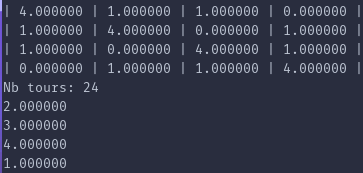
\includegraphics[scale=0.5]{./img/jacobi/jac_ex_1.png}

Voici la solution trouvée par \textbf{Gauss Seidel}:

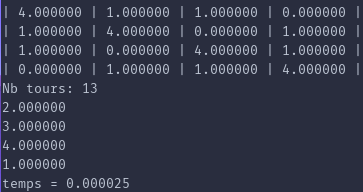
\includegraphics[scale=0.5]{./img/gauss_seidel/g_e_ex_1.png}

On constate que la solution trouvée avec les deux méthodes est la même et si on
regarde le nombre de tours effectués, on voit que \textbf{gauss-seidel} converge
presque deux fois plus vite que \textbf{jacobi}. Cependant, on constate tout de
même que le temps d’exécution du programme est presque le même. La solution
n'est pas arrondie, elle est exacte.\\

Résolvons le même système en faisant varier les valeurs dans b de $+0.005$:\\

Voici la solution trouvée par \textbf{Jacobi}:

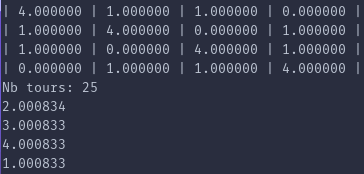
\includegraphics[scale=0.5]{./img/jacobi/jac_ex_1_mod.png}

Voici la solution trouvée par \textbf{Gauss Seidel}:

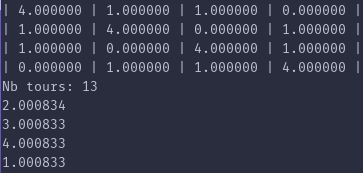
\includegraphics[scale=0.5]{./img/gauss_seidel/g_e_ex_1_mod.png}

On constate que les résultats ainsi que les temps d’exécution (légère variation
pour gauss seidel) et le nombre d'itérations n'ont pas beaucoup variés, donc la
modification effectuée sur b est bien gérée par le programme donc les méthodes
sont stables pour ce système.

\subsubsection{Autre système}

Résolution du système suivant:

\[
\begin{pmatrix}
  4 & 1 & -2\\
  -1 & 3 & 0\\
  -2 & -5 & 8\\
\end{pmatrix}X =
\begin{pmatrix}
  8\\
  3\\
  8\\
\end{pmatrix}
\]


Solutions trouvée par \textbf{Jacobi}:

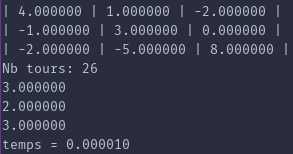
\includegraphics[scale=0.5]{./img/jacobi/jac_ex_4.png}\\

Solutions trouvée par \textbf{Gauss Seidel}:

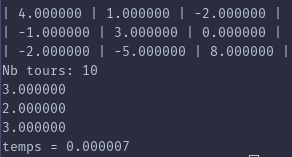
\includegraphics[scale=0.5]{./img/gauss_seidel/g_e_ex_4.png}\\

On constate encore une fois que \textbf{Jacobi} itère plus de fois que
\textbf{gauss seidel} mais que les temps d’exécution des deux programmes sont
toujours très proches. De plus, le programme trouve toujours une solution
précise.

Résolvons le même système en faisant varier les valeurs dans b de $+0.005$:\\

Voici la solution trouvée par \textbf{Jacobi}:

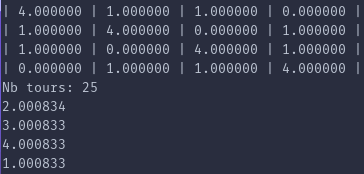
\includegraphics[scale=0.5]{./img/jacobi/jac_ex_1_mod.png}

Voici la solution trouvée par \textbf{Gauss Seidel}:

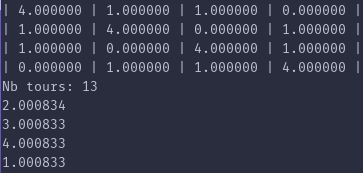
\includegraphics[scale=0.5]{./img/gauss_seidel/g_e_ex_1_mod.png}

On constate à nouveau la stabilité des méthodes sur cet exemple.

\subsubsection{Une Erreur}

Avec ce test, on voit que si la matrice ne respecte pas les contraintes requises
par les méthodes, celles-ci tournent à l'infini sans jamais converger vers la
solution du système (le programme s'arrête car la fonction est limitée à 100 tours).\\

Résolution de:

\[
\begin{pmatrix}
  1 & 2 & 1\\
  2 & 2 & 3\\
  5 & 1 & 8\\
\end{pmatrix} X =
\begin{pmatrix}
  2\\
  -1\\
  3\\
\end{pmatrix}
\]\\

Voici la solution trouvée par \textbf{jacobi}:

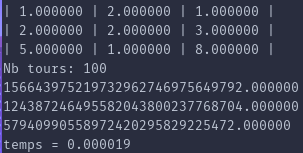
\includegraphics[scale=0.5]{./img/jacobi/jac_fail.png}

Voici la solution trouvée par \textbf{gauss seidel}:

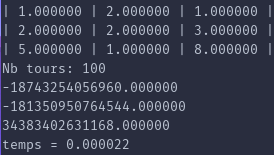
\includegraphics[scale=0.5]{./img/gauss_seidel/g_e_fail.png}

Les solutions trouvées sont incohérentes, les vraies solutions du système sont:
$x_{1} = \frac{76}{3} \approx 25,333333333$,
$x_{2} = \frac{-8}{3} \approx -2,666666667$ et
$x_{3} = \frac{-31}{3} \approx 10,333333333$


\subsection{Conclusion sur les méthodes itératives}

Le principal défaut de ces méthodes est qu'elles ne convergent pas pour tous les
systèmes, en effet, si la matrice n'est pas à diagonale dominante ou symétrique
et définie positive (pour Gauss Seidel), ces méthodes ne trouverons pas de
solutions au système et bouclerons à l'infini si le programme n'est pas prévu
pour s'arrêter à un nombre maximum d'itérations.
\\
\\
Cependant, ces deux méthodes sont bien plus précises que les méthodes directes
et sont donc efficaces pour palier au problème du manque de précision et
l'accumulation d'erreurs de calcul dues à l'utilisation des flottants dans les
ordinateurs du fait que la solution est améliorée à chaque itération. La
précision de la solution dépend de la précision demandée dans le programme qui
est limitée par la précision des flottants et la mémoire de l'ordinateur. A noter
que plus la précision demandée est élevée, plus le temps d’exécution sera grand,
cependant, en théorie, sans prendre en compte les faiblesses de la machine, si
les méthodes convergent, on peut obtenir une précision infinie.

\clearpage

%=============================================
%---------------annexes pour code-------------
%=============================================

\begin{appendix}
  \section*{Gauss}
  \lstinputlisting{./prog/gauss.c}
\end{appendix}
\clearpage

%=============================================

\begin{appendix}
  \section*{Cholesky}
  \lstinputlisting{./prog/cholesky.c}
\end{appendix}
\clearpage

%=============================================

\begin{appendix}
  \section*{Jacobi}
  \lstinputlisting{./prog/jacobi.c}
\end{appendix}
\clearpage

%=============================================

\begin{appendix}
  \section*{Gauss Seidel}
    \lstinputlisting{./prog/gauss_seidel.c}
\end{appendix}

\end{document}
